% !TEX root = ../thesis.tex
\iffalse
Results

    The results are actual statements of observations, including statistics, tables and graphs.
    Indicate information on range of variation.
    Mention negative results as well as positive. Do not interpret results - save that for the discussion. 
    Lay out the case as for a jury. Present sufficient details so that others can draw their own inferences and construct their own explanations. 
    Use S.I. units (m, s, kg, W, etc.) throughout the thesis. 
    Break up your results into logical segments by using subheadings
    Key results should be stated in clear sentences at the beginning of paragraphs.  It is far better to say "X had significant positive relationship with Y (linear regression p<0.01, r^2=0.79)" then to start with a less informative like "There is a significant relationship between X and Y".  Describe the nature of the findings; do not just tell the reader whether or not they are significant.  
\fi

\section{Pruning}
\subsection{Fully Connected Summation}
By applying distortions to remaining weights between training cycles, we have achieved the optimum result, where we have only one hidden node remaining. When we didn't apply the distortions, after the first training cycle, we couldn't find any nodes to prune. Using activation count and activation value statistics we fond an ideal solution in $7 \pm 2$ training cycles.

\subsection{MNIST Autoencoder}
In this setting we didn't see any change when we applied the distortions. When we applied L2 regularization on weights, we have seen some improvement in the number of nodes pruned and the final result. In the most ideal case, we have pruned our neural network from $1-32-64-32-1$ to $1-2-4-3-1$ nodes per layer. It took us $10\pm4$ training cycles to achieve these results. The loss we have achieved is very close to 0. 


\begin{figure}[h]
  \vspace{-45px}
  \centering
  \begin{subfigure}{.79\textwidth}
        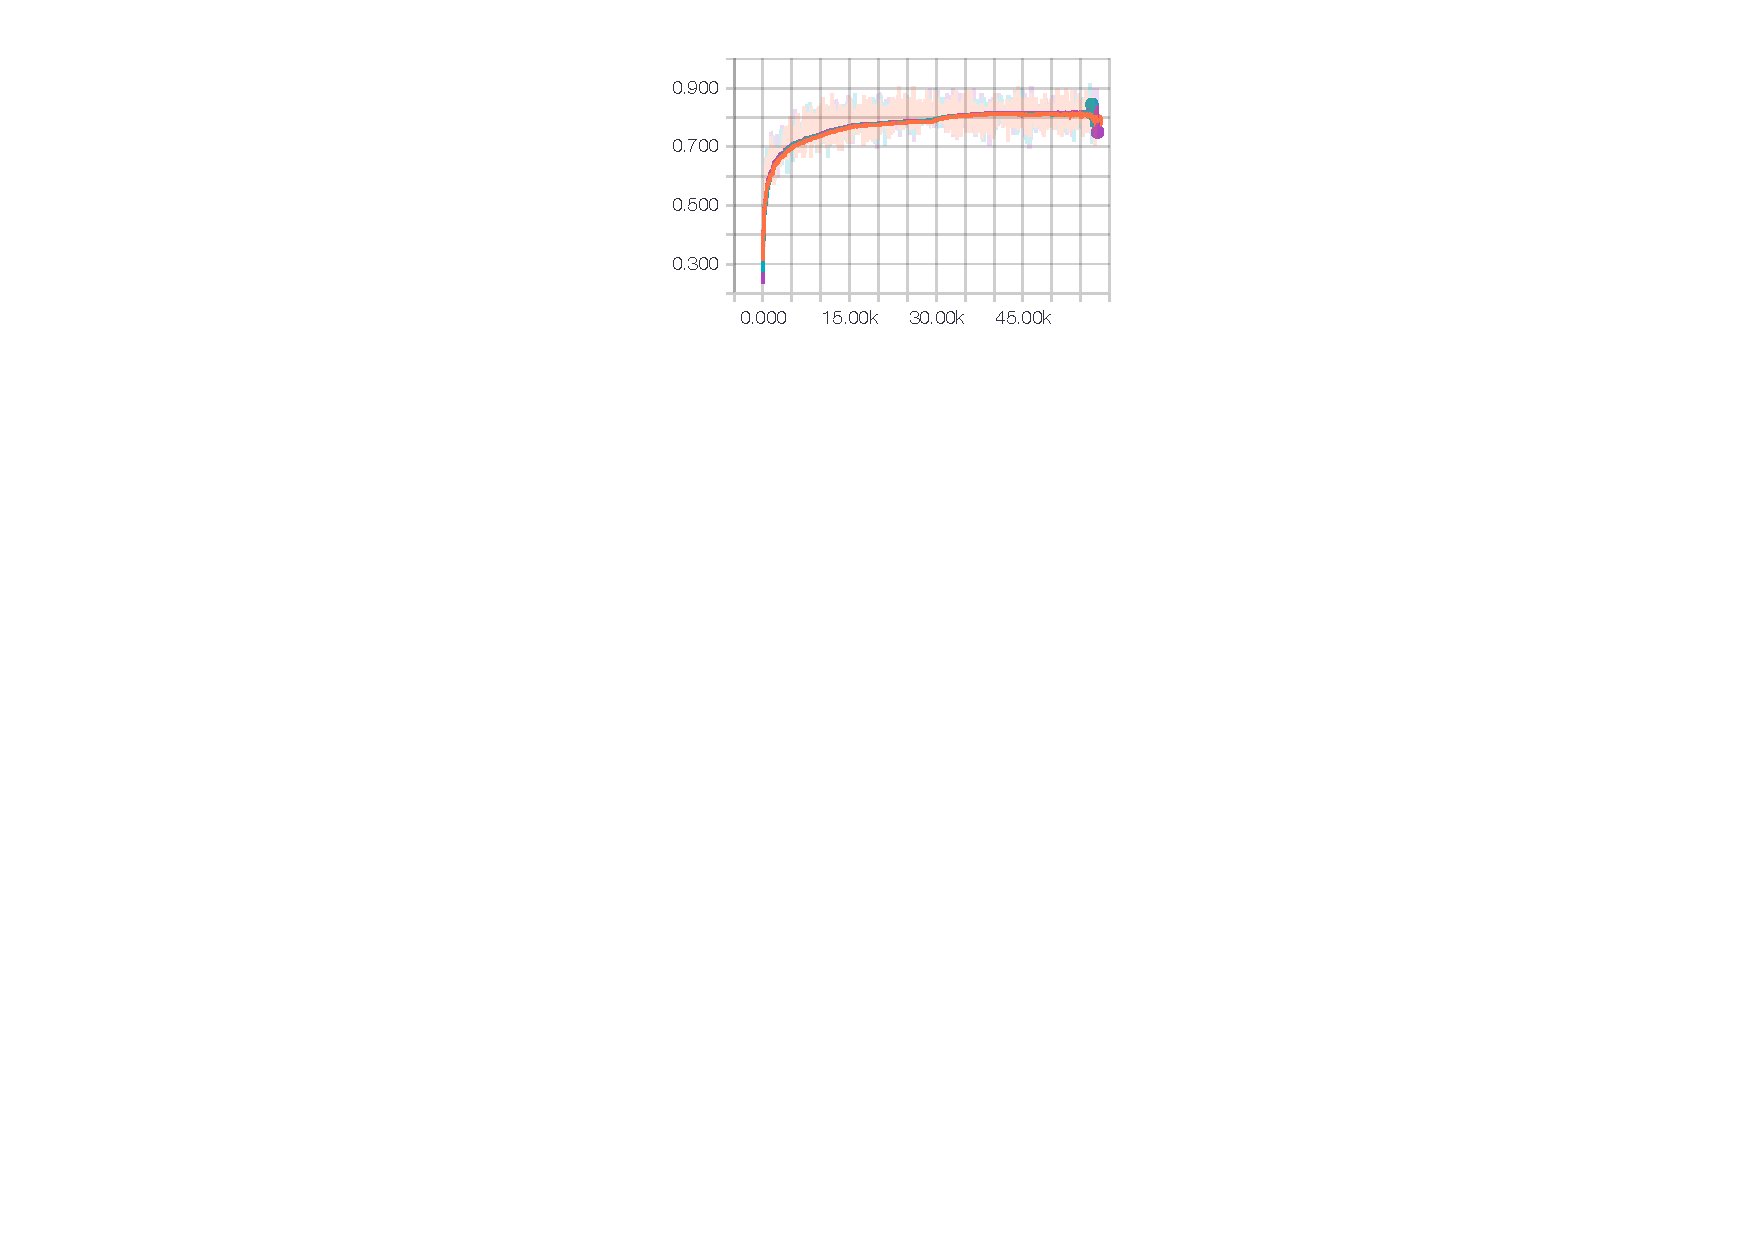
\includegraphics[width=1\linewidth]{images/convolution-comparison-test-dataset-full-accuracy.pdf}
        \caption{Smoothed top-1 accuracies in every step. For validation dataset.}
        \label{fig:conv-comparison-full}
  \end{subfigure}
  \begin{subfigure}{.79\textwidth}
        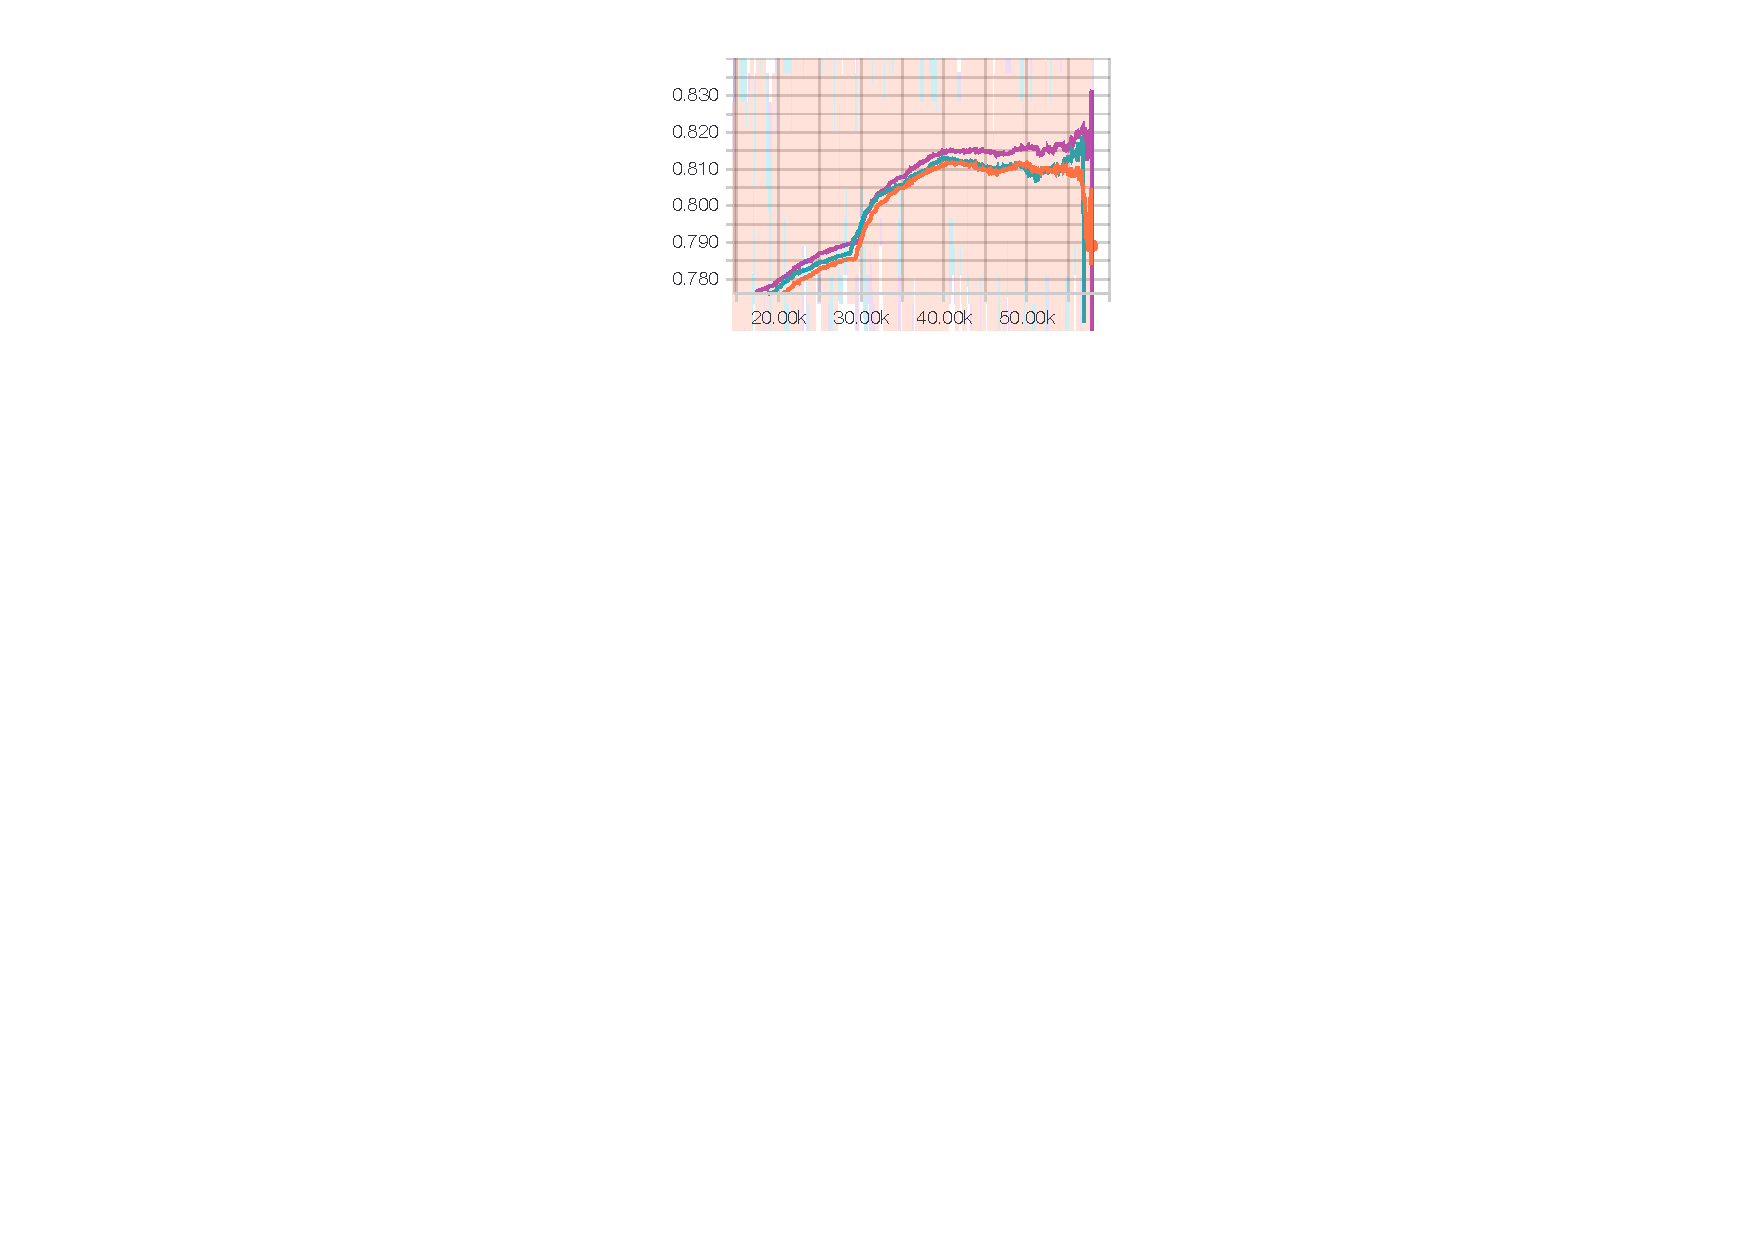
\includegraphics[width=1\linewidth]{images/convolution-comparison-test-dataset-accuracy-zoomed.pdf}
        \caption{Zoomed in version of Figure \ref{fig:conv-comparison-full}.}
  \end{subfigure}
  \begin{subfigure}{.49\textwidth}
        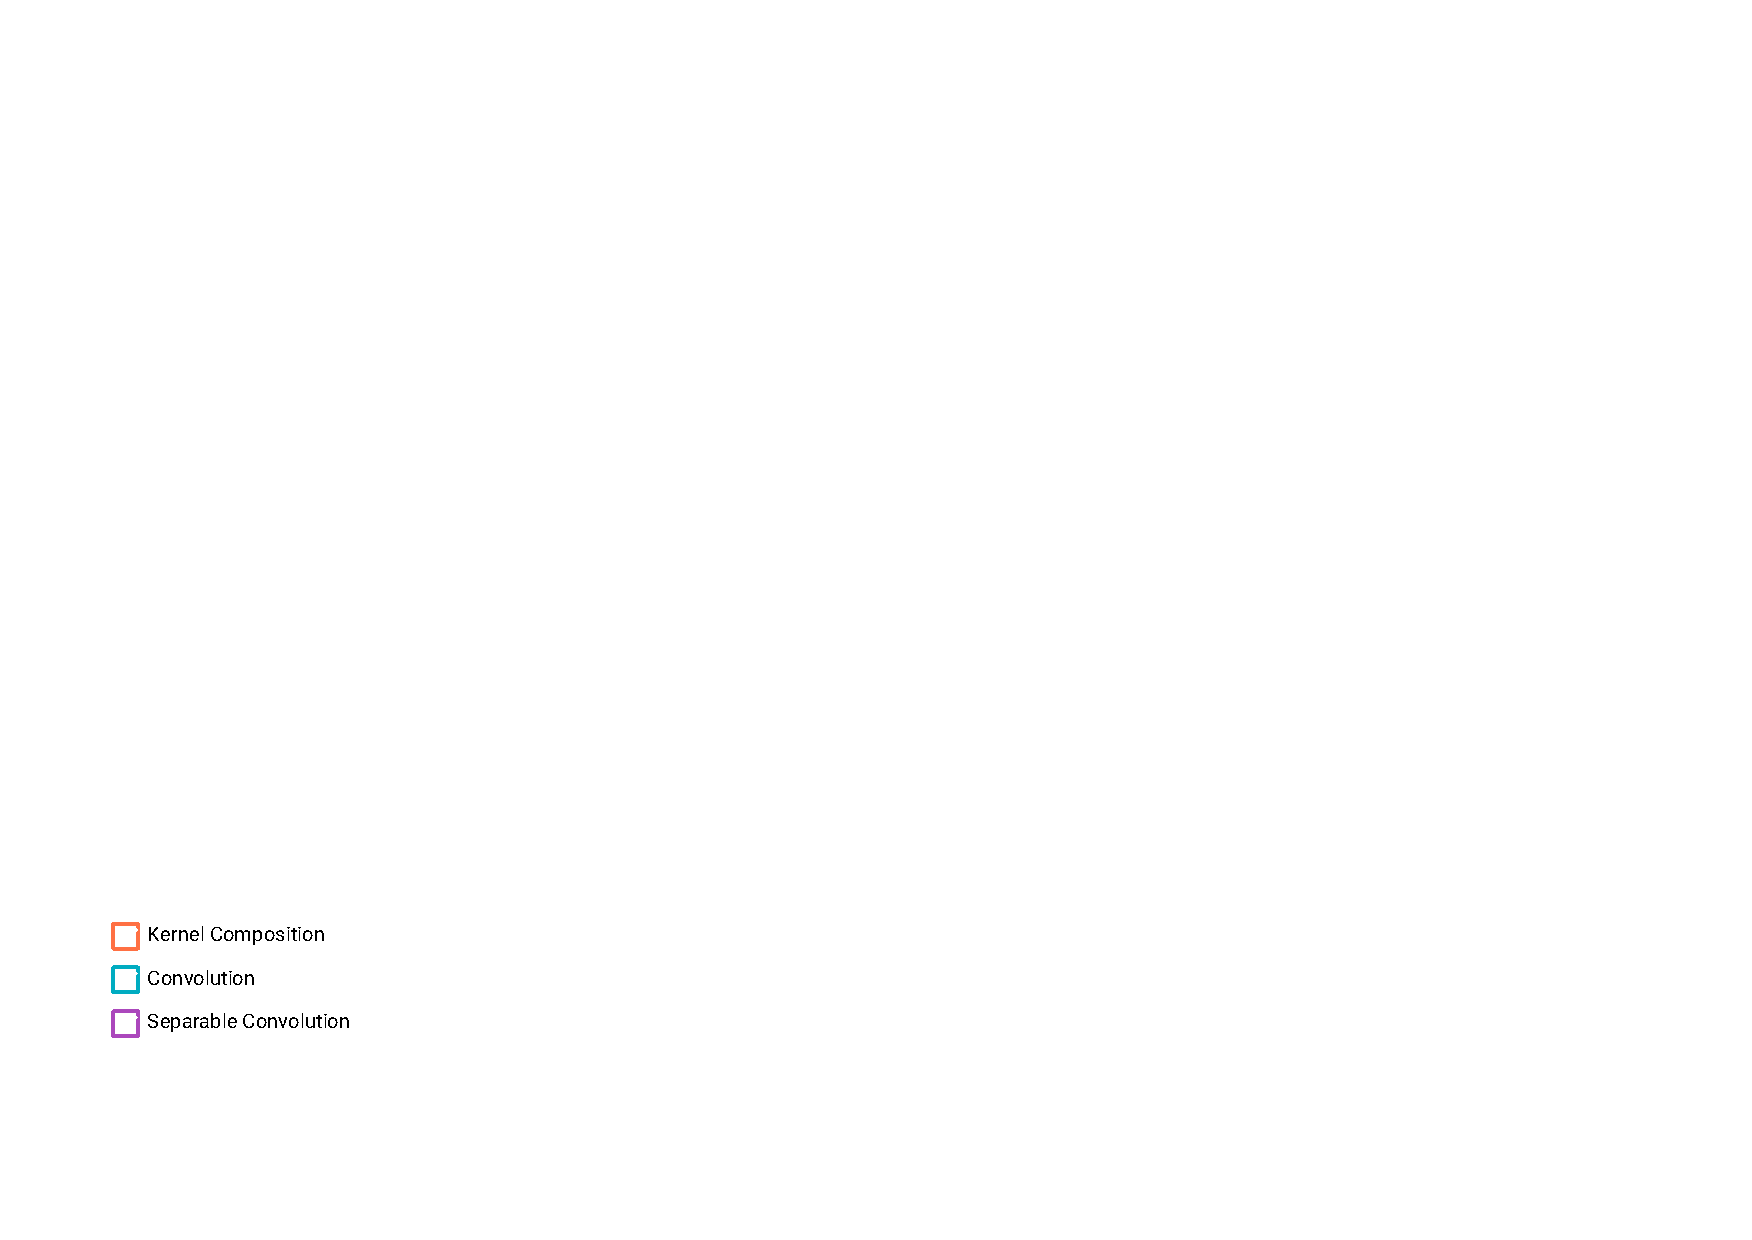
\includegraphics[width=1\linewidth]{images/convolution-comparison-legend.pdf}
        \caption{Color codes}
  \end{subfigure}
  \caption{Top-1 accuracy comparison of kernel composition, convolution and separable convolution operations. Accuracies for sub-samples of the validation dataset, compared after every training step. We see the thick lines representing smoothed values.}
  \label{fig:conv-comparison}
\end{figure}

\section{Convolution Operation Alternatives}
By comparing the convolution operation alternatives we try to figure out if separable or kernel composition methods can achieve similar performance to the convolution operation. In our experiments we have seen that kernel composing convolutions and convolutions are almost similar in terms of performance. We have seen that separable convolutions are slightly better than both operations. We have seen that separable convolutions achieve $82.3\%$ mean top-1 validation accuracy while regular convolutions achieve $81.6\%$ and kernel composing convolutions achieve $81.8\%$ in the whole validation dataset. Also in Figure \ref{fig:conv-comparison} we see the a validation performance comparison for these operations. 

\subsection{Non-Linearity in Separable Convolutions}
In our experiments we couldn't see any difference between adding non-linear separable convolutions and separable convolutions. 

\subsection{Proposed First Convolutional Layer}
In our experiments we didn't see many differences in terms of accuracy. Even tho our proposed method starts a bit better, both converge on $85\%$ top-1 accuracy. 
\begin{figure}[h]
  \vspace{-45px}
  \centering
  \begin{subfigure}{.79\textwidth}
        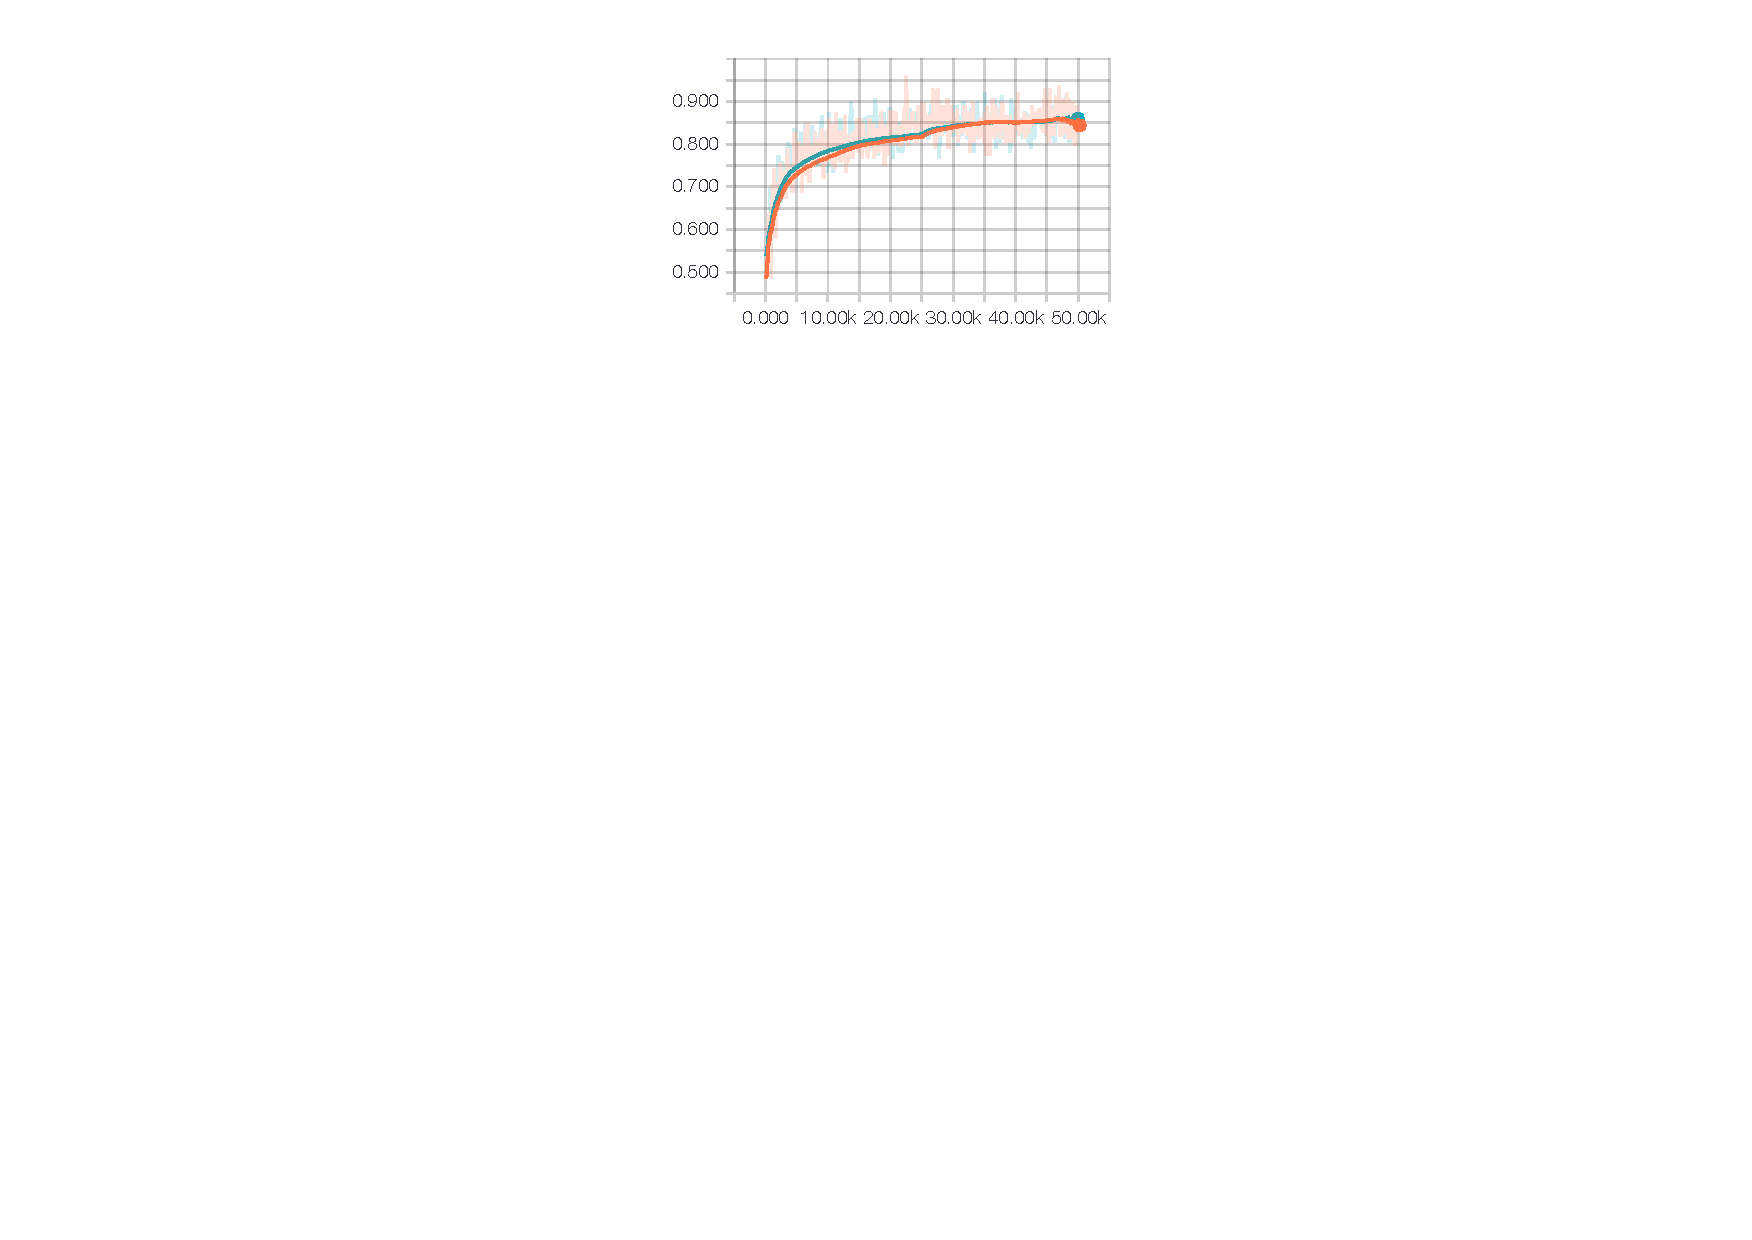
\includegraphics[width=1\linewidth]{images/proposed_conv_comparison_evaluation.pdf}
        \caption{Smoothed top-1 accuracies in every step. For samples from validation dataset.}
        \label{fig:conv-comparison-proposed-full}
  \end{subfigure}
  \begin{subfigure}{.79\textwidth}
        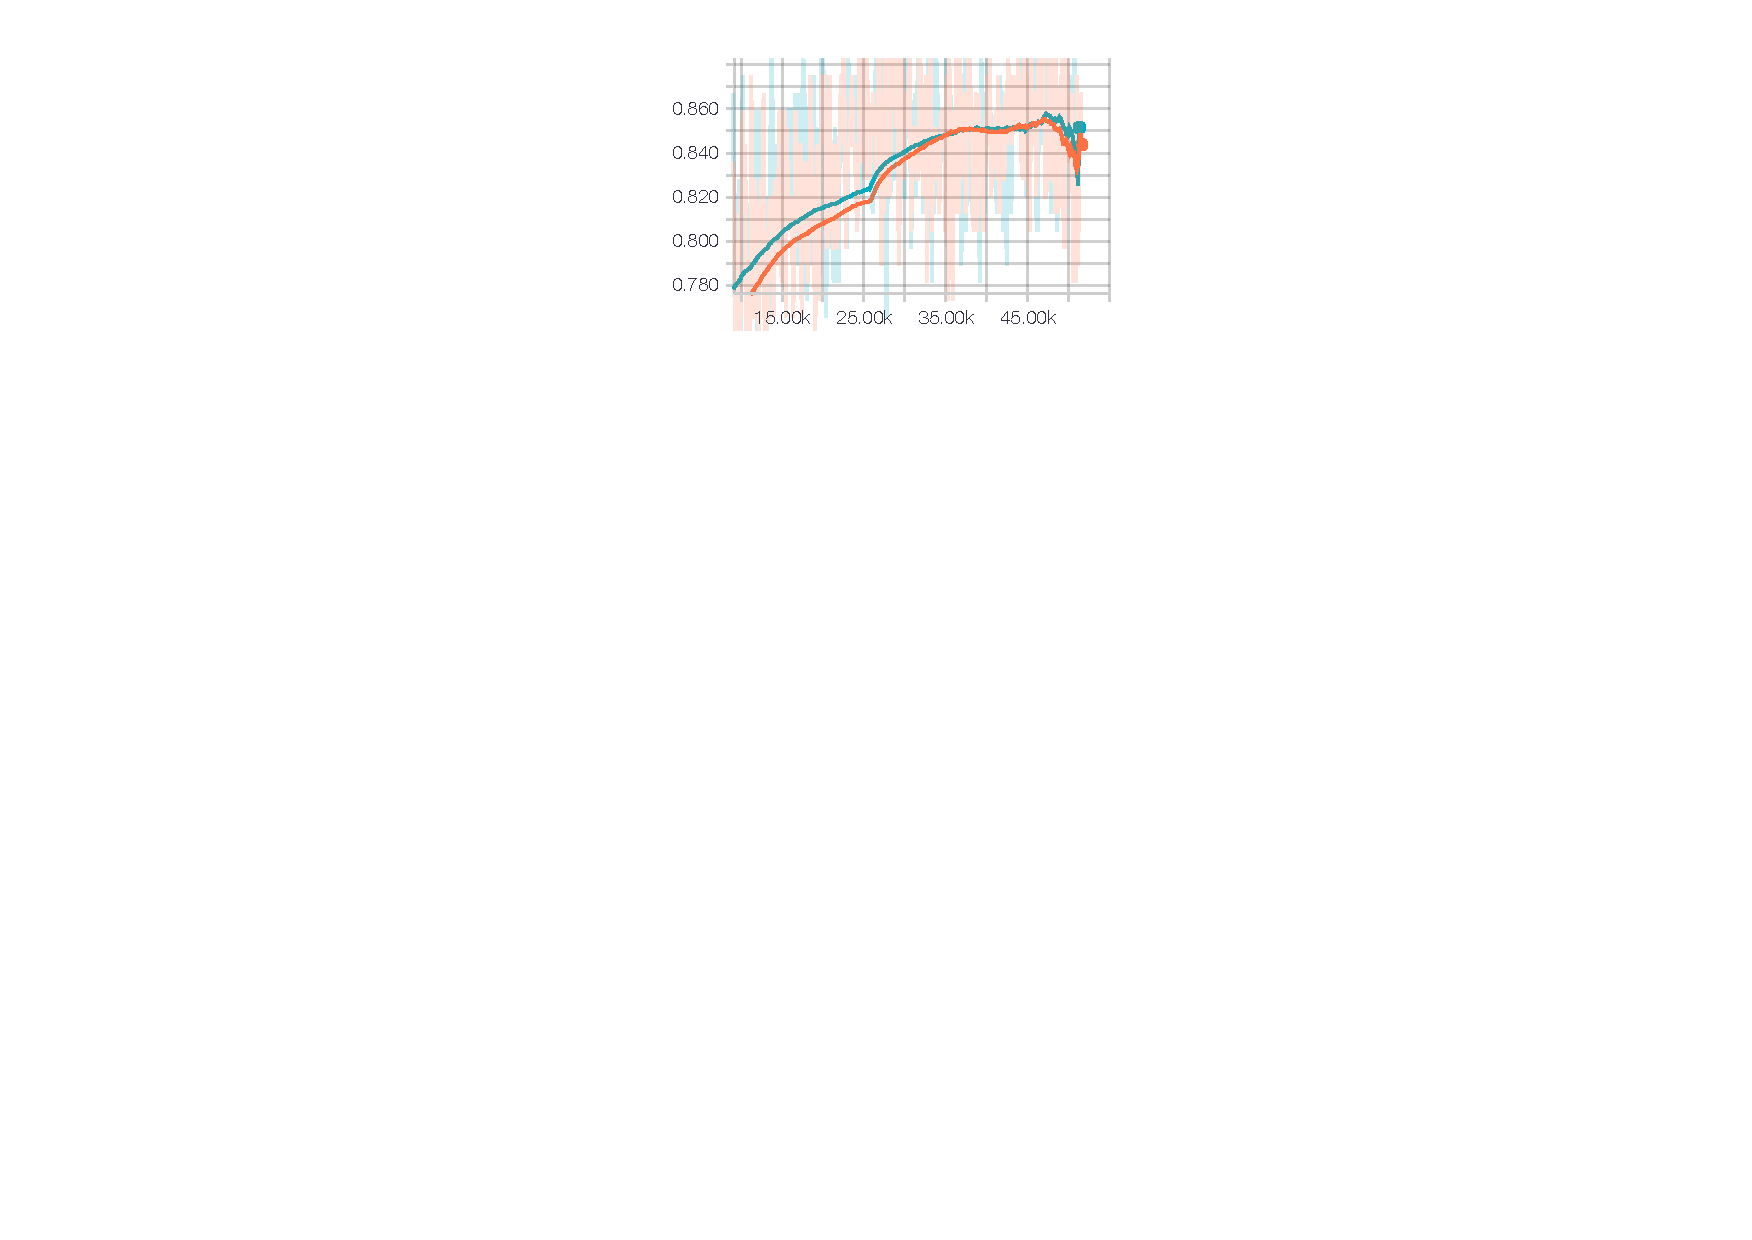
\includegraphics[width=1\linewidth]{images/proposed_conv_comparison_evaluation_zoomed.pdf}
        \caption{Zoomed in version of Figure \ref{fig:conv-comparison-proposed-full}.}
  \end{subfigure}
  \begin{subfigure}{.49\textwidth}
        
\includegraphics[width=1\linewidth]{images/proposed_conv_legend.pdf}
        \caption{Color codes}
  \end{subfigure}
  \caption{Top-1 accuracy comparison of 7 by 7 convolution and our proposed convolution as the first layer(s) of the model. Accuracies for sub-samples of the validation dataset, compared after every training step. We see the thick lines representing smoothed values.}
  \label{fig:proposed-comparison}
\end{figure}

\section{Benchmarks}
We have benchmarked 20 models in different sizes and shapes. 
\todoin{plot a graph showing the difference between the model size and cpu utilization} 




